%! Author = salom
%! Date = 18.09.2020
\chapter{Experimental Evaluation}\label{ch:evaluation}

We tested our implementation of the strengthened potential heuristics on 1827 STRIPS problems with the official domains from the International Planning Competition (IPCs).
Further, we used Downward Lab~\citep{seipp-et-al-zenodo2017} to set up the tests and ran them on the sciCORE high-performance computing infrastructure.
We set the time limit for each problem to 30 minutes and the memory limit to 8 GB.
The different heuristics were all used in an $\textup{A}^{\star}$ search~\citep{hart1968formal}.

We test whether the LP constraints built with disambiguations improve performance and compare the different optimization functions against each other.
Further, we compare different ensemble heuristics and their respective amount of heuristics used, as well as the additional constraints on the initial state and on random states.
Last, we compare our results to the results from the evaluation of~\cite{fivser2020strengthening}.

We refer to the compared variants of heuristics as follows:

\begin{center}
    \begin{tabularx}{\textwidth}{@{}lX@{}}
        \textbf{\texttt{lmc}}: & The LM-Cut heuristic, introduced by~\cite{helmert-domshlak-icaps2009}. \\
        \textbf{\texttt{init}}: & The initial state potential heuristic (Eq.~\eqref{eq:initial-state}). \\
        \textbf{\texttt{all}}: & The all states potential heuristic (Eq.~\eqref{eq:all-states}). \\
        \textbf{\texttt{max}}: & The maximization over \texttt{init} and \texttt{all}. \\ %% max_AI
        \textbf{\texttt{div}}: & The diversification heuristic~\citep{seipp2015new} with 1000 samples. \\
        \textbf{$\texttt{S}_\texttt{i}^\texttt{n}$}: & The sample based potential heuristic (Eq.~\eqref{eq:uniform-opt}), $n$ being the number of heuristics and $i$ the number of samples per heuristic. \\ %% S_1^100 = S, S_1000^1 = S_.N
        \textbf{$\texttt{M}_\texttt{k}$}: & The strengthened all states potential heuristic with $\mathrm{opt}^k_\mathcal{M}$ (Eq.~\eqref{eq:opt1}). \\
        \textbf{$\texttt{K}_\texttt{k}^\texttt{n}$}: & The strengthened ensemble potential heuristic with $\mathrm{opt}^{t,k}_\mathcal{M}$ (Eq.~\eqref{eq:opt2}) with $|t|=1$ and $n$ heuristics. \\
        \textbf{$\texttt{L}_\texttt{k}^\texttt{n}$}: & The same as $\texttt{K}_\texttt{k}^\texttt{n}$, but with $|t|=2$. \\
        \textbf{$\texttt{J}_\texttt{k}^\texttt{n}$}: & The same as $\texttt{K}_\texttt{k}^\texttt{n}$, but with $|t|=3$. \\
    \end{tabularx}
\end{center}

In addition, \textbf{\texttt{N}} refers to the non-strengthened LP, while \textbf{\texttt{D}} uses the LP strengthened with disambiguations.
When the additional constraint on the initial state is used, \textbf{\texttt{I}} is appended to the name of the heuristic and \textbf{\texttt{R}} if the constraints on random states are used.

The attributes we use to compare different configurations are:

\begin{center}
    \begin{tabularx}{\textwidth}{@{}lX@{}}
        \textbf{Coverage}: & The amount of problems solved with the respective configuration. \\
        \textbf{Expansions}: & The number of state expansions needed to solve the problem. \\
        \textbf{Total Time}: & The total time needed to solve the problems without pre processing, in minutes. \\
        \textbf{Search Time}: & The time needed for the search only, in minutes. \\
        \textbf{Out of Memory}: & The amount of problems which failed due to a lack of memory. \\
        \textbf{Out of Time}: & The amount of problems which failed due to a lack of time. \\
    \end{tabularx}
\end{center}

The attributes expansions, total time and search time are the geometric mean over all problems which were solved by all configurations.
The search time is exclusively the time needed to perform the search.
In all tables, the best value per attribute is written in bold.
For coverage, this is the highest value and for the other attributes it is the lowest.

\section{Results}\label{sec:results}
The following table shows results for the heuristics which were already provided in the Fast Downward planning system.

\begin{table}[h!]
    \begin{center}
        \begin{tabular}{|r|c|c|c|c|c|c|c|}
            \hline
            & \textbf{\texttt{lmc}} & \textbf{\texttt{all-N}} & \textbf{\texttt{init-N}} & \textbf{\texttt{max-N}} & \textbf{\texttt{div-N}} & \textbf{$\texttt{S}_\texttt{1}^\texttt{100}$\texttt{-N}} & \textbf{$\texttt{S}_\texttt{1000}^\texttt{1}$\texttt{-N}} \\
            \hline \hline
            \textbf{Coverage}       & 958           & 929           & 891   & 948   & \textbf{963}  & 945   & 961   \\ \hline
            \textbf{Expansions}     & \textbf{1287} & 10244         & 22415 & 8270  & 6904          & 7181  & 9238  \\ \hline
            \textbf{Total Time}     & 0.57          & \textbf{0.29} & 0.54  & 0.33  & 0.74          & 0.94  & 0.33  \\ \hline
            \textbf{Search Time}    & 0.52          & 0.23          & 0.43  & 0.24  & 0.74          & 0.94  & \textbf{0.22}  \\ \hline
            \textbf{Out of Memory}  & \textbf{0}    & 870           & 911   & 854   & 623           & 170   & 844   \\ \hline
            \textbf{Out of Time}    & 852           & 11            & 8     & 8     & 224           & 695   & \textbf{5}     \\ \hline
        \end{tabular}
        \caption{Test results for the already provided heuristics.}
        \label{table:standard_heuristics}
    \end{center}
\end{table}

We see that \texttt{lmc}, \texttt{div-N} and $\texttt{S}_\texttt{1000}^\texttt{1}$\texttt{-N} have the highest coverage over all problems.
Further, \texttt{lmc} has the lowest number of expansions and therefore the lowest out of memory errors.
$\texttt{S}_\texttt{1000}^\texttt{1}$\texttt{-N}, on the other hand, is the fastest of the three configurations and has only few out of time errors.

As the same search algorithm is used for all configurations, the number of expansions can be used as an indicator for the quality of the heuristic value.
Few expansions combined with a high coverage, e.g. with \texttt{lmc}, can be interpreted as an efficient search, with only few state expansions, due to a good heuristic value.

In the following subsections, we compare these results to the results we obtained with the features we implemented.

\subsection{Mutex Based Linear Program}\label{subsec:mutex-based-linear-program}
First, we compare the results from above with the ones obtained with the LP built with mutexes and disambiguations.
The following table shows multiple configurations and their respective results.

\begin{table}[h!]
    \begin{center}
        \begin{tabular}{|r|c|c|c|c|c|c|}
            \hline
            & \textbf{\texttt{all-D}} & \textbf{\texttt{init-D}} & \textbf{\texttt{max-D}} & \textbf{\texttt{div-D}} & \textbf{$\texttt{S}_\texttt{1}^\texttt{100}$\texttt{-D}}& \textbf{$\texttt{S}_\texttt{1000}^\texttt{1}$\texttt{-D}}\\
            \hline \hline
            \textbf{Coverage}       & 879   & 881           & 932   & 837           & 853           & \textbf{952}  \\ \hline
            \textbf{Expansions}     & 12101 & 18964         & 7863  & \textbf{5269} & 5503          & 7697          \\ \hline
            \textbf{Total Time}     & 0.68  & 0.90          & 0.84  & 4.18          & 3.29          & \textbf{0.64} \\ \hline
            \textbf{Search Time}    & 0.27  & 0.39          & 0.24  & \textbf{0.19} & 0.31          & \textbf{0.19} \\ \hline
            \textbf{Out of Memory}  & 824   & 824           & 770   & 560           & \textbf{273}  & 726           \\ \hline
            \textbf{Out of Time}    & 75    & \textbf{73}   & 76    & 381           & 652           & 100           \\ \hline
        \end{tabular}
        \caption{Test results for mutex based Linear Programs.}
        \label{table:mutex_lp}
    \end{center}
\end{table}

The coverage is lower for these configurations.
However, the number of expansions is better for all configurations with respect to their non-mutex version, except for \texttt{all}.
The scatter plot~\ref{fig:N_D_exp} shows how the the amount of expansions differ between the two different LPs for all solved problems for \texttt{all} and $\texttt{S}_\texttt{1000}^\texttt{1}$.
Dots above the diagonal represent problems for which \texttt{D} has more expansions, dots below the diagonal represent problems for which \texttt{N} has more expansions.
For \texttt{all}, more dots are above the diagonal, as it has a higher number of expansions.
For $\texttt{S}_\texttt{1000}^\texttt{1}$, more dots are below the diagonal.

\begin{figure}[h!]
\centering
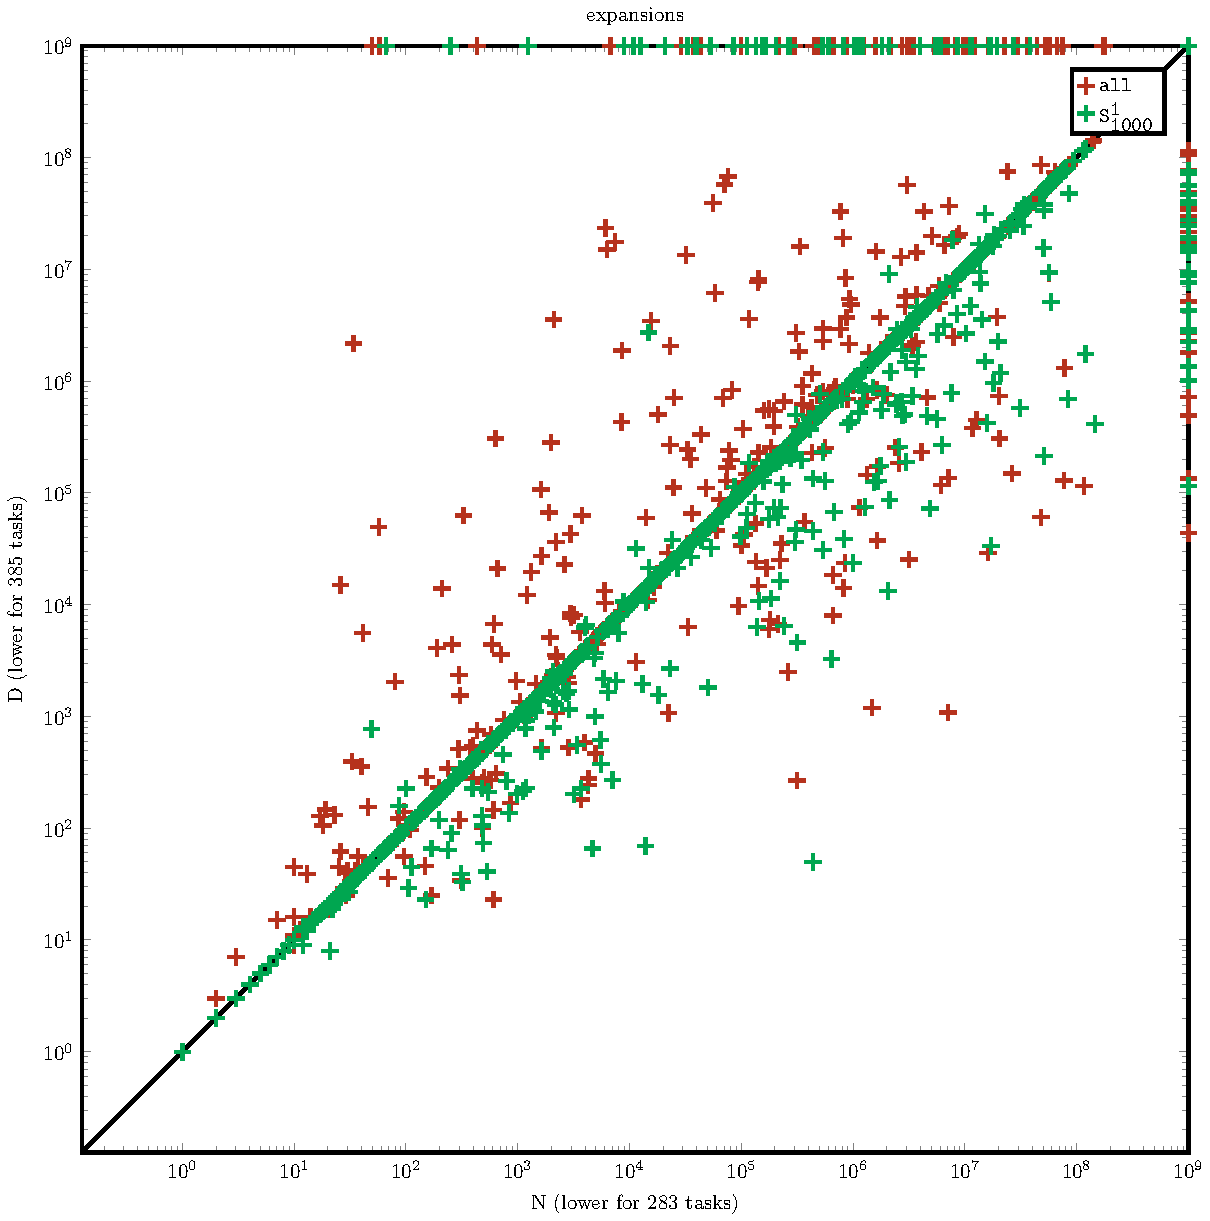
\includegraphics[width=0.6\textwidth]{N_D_exp}
\caption{Number of expansions of \texttt{all} and $\texttt{S}_\texttt{1000}^\texttt{1}$ for both LPs per problem.}
\label{fig:N_D_exp}
\end{figure}

Due to the smaller amount of expanded states, less out of memory errors occur.
The number of out of time errors, on the other hand, are higher.
This is no surprise, as the total time is higher for all configurations as well.
The search time is roughly the same, which indicates that the building of the mutex table and the mutex based LP is the most time consuming difference.
Hence, it is the reason for the high amount of out of time errors and the relatively low coverage.
This holds especially for \texttt{div-D} and $\texttt{S}_\texttt{1}^\texttt{100}$\texttt{-D}, where the total time is much higher than before and the difference between total and search time is immense.
The search itself is a lot faster, which indicates good heuristic values.
Both heuristics build the LP multiple times and, in our implementation, each time the mutex table needs to be computed from a fresh start.

We already greatly enhanced the performance of building the mutex table.
However, finding a more efficient way for building the mutex table would lead to a higher coverage.
To build the mutex table, we optimized the (very slow) Fast Downward hm-heuristic for $m=2$ and ignored heuristic values, as we are only interested in the binary reachability.
Before the optimization, the mutex table was built for 1450 problems, in 117 seconds on average.
Now, 1776 mutex tables are built in 34 seconds on average.
Thus, over 300 additional mutex tables can be built in less than 30 minutes, some of them in less than 20 seconds.

Comparing the configurations amongst each other, we see that the coverages of $\texttt{S}_\texttt{1000}^\texttt{1}$\texttt{-D} and \texttt{max-D} are still good, as they only decrease by around 10 problems.
So does the coverage of \texttt{init}.
These are also the configurations, for which the expansions and search time sunk, as well as the out of memory errors.
The other configurations are significantly worse with disambiguations.
This does not hold for mutex based optimization functions.

\subsection{Mutex Based Optimization Functions}\label{subsec:mutex-based-optimization-functions}
The next table shows the results for our mutex based optimization functions.
For the ensemble heuristics (\texttt{K}, \texttt{L} and \texttt{J}), we chose $n=10$, since using 10 heuristics gave the best results on average (\autoref{table:ensemble-n}).
\begin{table}[h!]
    \begin{center}
        \begin{tabular}{|r|c|c|c|c|c|c|c|c|c|}
            \hline
            & \textbf{$\texttt{M}_\texttt{1}$\texttt{-D}} & \textbf{$\texttt{M}_\texttt{2}$\texttt{-D}} & \textbf{$\texttt{K}_\texttt{1}^\texttt{10}$\texttt{-D}} & \textbf{$\texttt{K}_\texttt{2}^\texttt{10}$\texttt{-D}} & \textbf{$\texttt{L}_\texttt{1}^\texttt{10}$\texttt{-D}} & \textbf{$\texttt{L}_\texttt{2}^\texttt{10}$\texttt{-D}} & \textbf{$\texttt{J}_\texttt{1}^\texttt{10}$\texttt{-D}} & \textbf{$\texttt{J}_\texttt{2}^\texttt{10}$\texttt{-D}}\\
            \hline \hline
            \textbf{Coverage}       & 900           & 859           & 911   & 831   & 921   & 840   & \textbf{922}  & 845   \\ \hline
            \textbf{Expansions}     & 8297          & 8240          & 6790  & 6847  & 6126  & 6273  & 6197          & \textbf{6039} \\ \hline
            \textbf{Total Time}     & \textbf{0.59} & 1.23          & 0.89  & 4.23  & 0.99  & 3.93  & 1.02          & 3.20  \\ \hline
            \textbf{Search Time}    & \textbf{0.20} & \textbf{0.20} & 0.86  & 4.08  & 0.86  & 3.78  & 0.89          & 3.04  \\ \hline
            \textbf{Out of Memory}  & 802           & 726           & 714   & 608   & 691   & 589   & 677           & \textbf{586}   \\ \hline
            \textbf{Out of Time}    & \textbf{77}   & 203           & 155   & 351   & 169   & 364   & 193           & 364   \\ \hline
        \end{tabular}
        \caption{Test results for mutex based potential heuristics.}
        \label{table:mutex_based_heuristics}
    \end{center}
\end{table}

For the four different categories, \texttt{M}, \texttt{K}, \texttt{L} and \texttt{J}, we see that the configurations with smaller $k$ are always  better.
This is due to the higher time and memory consumption needed for bigger extensions, which can be concluded from the increasing sum of out of time and out of memory failures.
We can also see that extending partial states by two facts is more time consumptive, as more out of time errors occur for these configurations.
Our pretests showed, that for $k=3$ the coverage decreases about 30\% compared to $k=1$.
For even higher $k$, it would drop vastly, as the memory and time limits are not high enough to extend (multiple) partial states to this size.

Currently, the implementation for mutex based potential heuristics is able to work with any $k\in \mathbb{N}$ smaller than the size of a state.
An optimization for $k=1$ and $k=2$ could, similarly to the optimization of building the mutex table, enhance the coverage as well.

However, the fact that the amount of expansions decreases for greater $k$ and $t$ shows that the approach for mutex based potential heuristics is good.
For $|t|=3$, the coverage and the number of expansions are better than for smaller $t$.

The comparison of the results for mutex based potential functions with Table~\ref{table:standard_heuristics} shows that the coverage is not higher than for any of the former configurations.
However, less out of memory errors occurred, while the out of time errors increased.
This is, similar to the results for the mutex based LP (Sec.~\ref{subsec:mutex-based-linear-program}), due to the building of the mutex table.

We also tested the configurations $\texttt{M}_\texttt{1}$\texttt{-N} and $\texttt{M}_\texttt{2}$\texttt{-N}, which have a slightly higher coverage.
With the non-mutex based LP, the number of expansions and therefore the amount of out of memory errors are higher.
The higher coverage is due to the saved effort by not considering mutexes for building LP.

\subsection{Ensemble Heuristics}\label{subsec:mutex-based-ensemble-heuristics}
Table~\ref{table:ensemble-n} shows the coverage for different sample based ensemble heuristics, for different amounts of used heuristics.

\begin{table}[h!]
    \begin{center}
        \begin{tabular}{|r|c|c|c|c|c|c|}
            \hline
            \textbf{\texttt{n}} & \textbf{5} & \textbf{10} & \textbf{50} & \textbf{100} & \textbf{250} & \textbf{500} \\
            \hline \hline
            \textbf{$\texttt{S}_\texttt{1}$} & \textbf{889} & 888 & 867 & 852 & 815 & 773 \\ \hline
            \textbf{$\texttt{K}_\texttt{1}$} & 904 & \textbf{911} & 896 & 861 & 790 & 747 \\ \hline
            \textbf{$\texttt{K}_\texttt{2}$} & 835 & 831 & \textbf{888} & 865 & 669 & 615 \\ \hline
            \textbf{$\texttt{L}_\texttt{1}$} & 911 & \textbf{921} & 884 & 856 & 771 & 734 \\ \hline
            \textbf{$\texttt{L}_\texttt{2}$} & \textbf{840} & \textbf{840} & 796 & 756 & 670 & 615 \\ \hline
        \end{tabular}
        \caption{Comparison over different \texttt{n} for different ensemble heuristics.}
        \label{table:ensemble-n}
    \end{center}
\end{table}

The best results are achieved with smaller $n$.
In fact, the best coverage, 921, is achieved with $\texttt{L}_\texttt{1}^\texttt{10}$.

However, the number of expansions decrease with increasing $n$, indicating that the ensemble heuristics are more accurate when using more heuristics.
But the more heuristics are used, the more out of time errors occur.
This is both because more heuristics need to be computed and because they all need to be considered for each state which is evaluated.

The absolute numbers in Table~\ref{table:ensemble-n} should be taken with a grain of salt, as they are produced with randomness and differ for each run.
Running the tests multiple times shows that $n=5$ is too small, as the variety of generated samples is not big enough to produce good results.
For $n=50$ on the other hand, the time consumption of computing all heuristics is to high.
Further tests would be necessary, to see whether $n=10$ really is the sweet spot, or if it lies somewhere else in between 5 and 50
\newpage

\subsection{Additional Constraint on the Initial State}\label{subsec:additional-constraint-on-the-initial-state}
The best coverage for all configurations is obtained with the additional constraints on the initial state.

\begin{table}[h!]
    \begin{center}
        \begin{tabular}{|r|c|c|c|c|c|}
            \hline
            & \textbf{\texttt{all-N-I}} & \textbf{\texttt{div-N-I}} & \textbf{$\texttt{S}_\texttt{1000}^\texttt{1}$\texttt{-N-I}} & \textbf{$\texttt{M}_\texttt{1}$\texttt{-D-I}} & \textbf{$\texttt{M}_\texttt{2}$\texttt{-D-I}} \\
            \hline \hline
            \textbf{Coverage}       & \textbf{965}  & 956   & 963       & 950           & 906 \\ \hline
            \textbf{Expansions}     & 8532          & 7741  & 9040      & 6585          & \textbf{6561} \\ \hline
            \textbf{Total Time}     & \textbf{0.27} & 0.70  & 0.33      & 0.60          & 1.21 \\ \hline
            \textbf{Search Time}    & 0.21          & 0.70  & 0.21      & \textbf{0.17} & \textbf{0.17} \\ \hline
            \textbf{Out of Memory}  & 837           & 716   & 843       & 729           & \textbf{705} \\ \hline
            \textbf{Out of Time}    & 8             & 127   & \textbf{4}& 115           & 183 \\ \hline
        \end{tabular}
        \caption{Test results for the additional constraint on the initial state.}
        \label{table:initial-constraint}
    \end{center}
\end{table}

None of the configurations shows a higher total time nor search time than before, despite the fact that the LP is solved twice.
First, to optimize the heuristic value for the initial state, then for the actual optimization function.
In addition, the number of expansions is smaller than before, and less time and memory errors occur in total.
The plots~\ref{fig:exp_all} and~\ref{fig:search_all} show very nicely how the number of expansions and the search time is smaller for \texttt{all-N-I}, compared to \texttt{all-N}.

\begin{figure}[h!]
\centering
    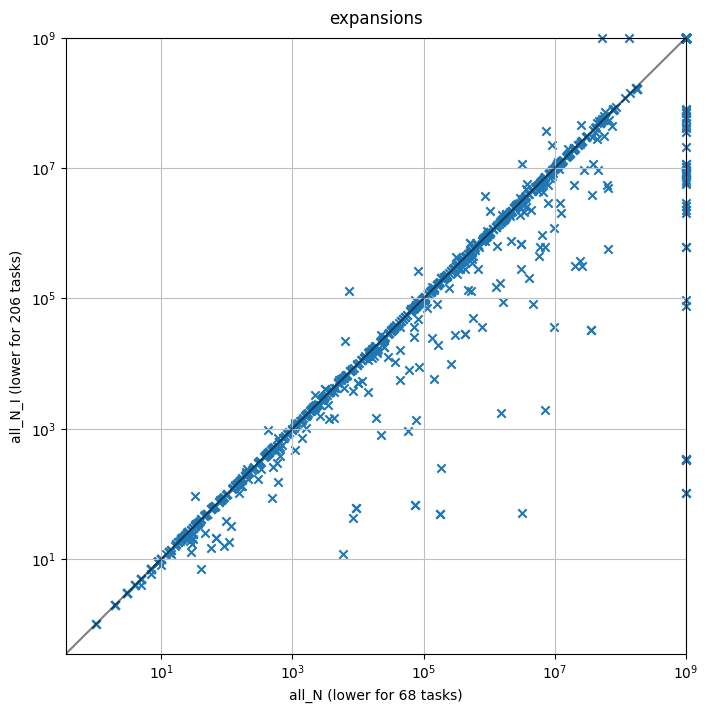
\includegraphics[width=0.5\textwidth]{all_I_exp}
    \caption{Number of expansions for \texttt{all} for both LPs per problem}
    \label{fig:exp_all}
\end{figure}

\begin{figure}[h!]
\centering
    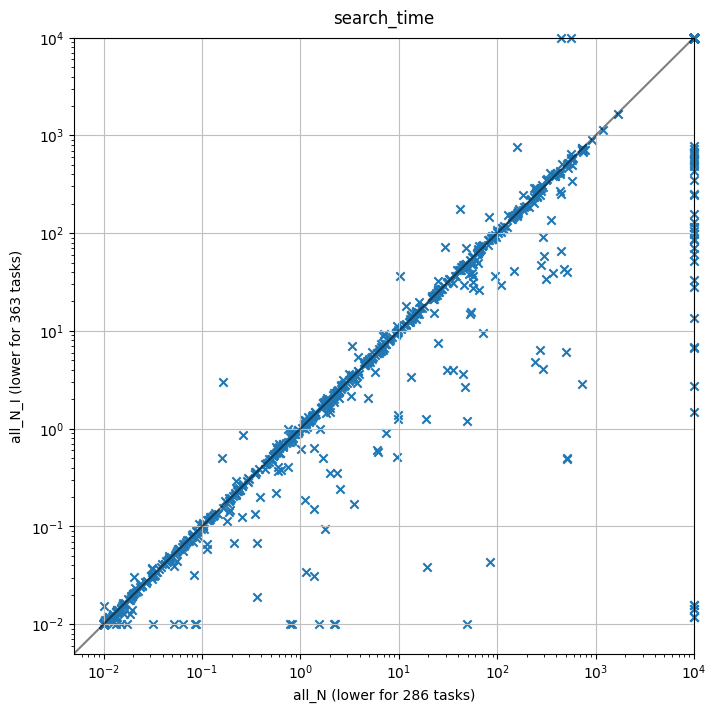
\includegraphics[width=0.5\textwidth]{all_I_search}
    \caption{Search Time  for \texttt{all} for both LPs per problem}
    \label{fig:search_all}
\end{figure}

It is remarkable, that \texttt{all-N-I} has a better coverage than \texttt{max-N} (948).
Presumably, \texttt{max} chooses \texttt{init} for states which are close to the initial state and \texttt{all} otherwise.
\texttt{all-N-I} on the other hand has high heuristic values on average, with a main focus on on the initial state.
This results in two very similar heuristics.
The higher coverage of \texttt{all-N-I} is due to its lower time consumption.
The configuration \texttt{max-N} takes longer to compute, as it must generate two independent LPs.
It takes less effort, to build an LP, solve it and then resolve it, as \texttt{all-N-I} does, since the presolving of the LP is only done once.
As plot~\ref{fig:search_max_all} shows, the search time is much lower for \texttt{all-N-I} than for \texttt{max}.
This is because \texttt{max} must consider two heuristics for each evaluated state.

\begin{figure}[h!]
\centering
    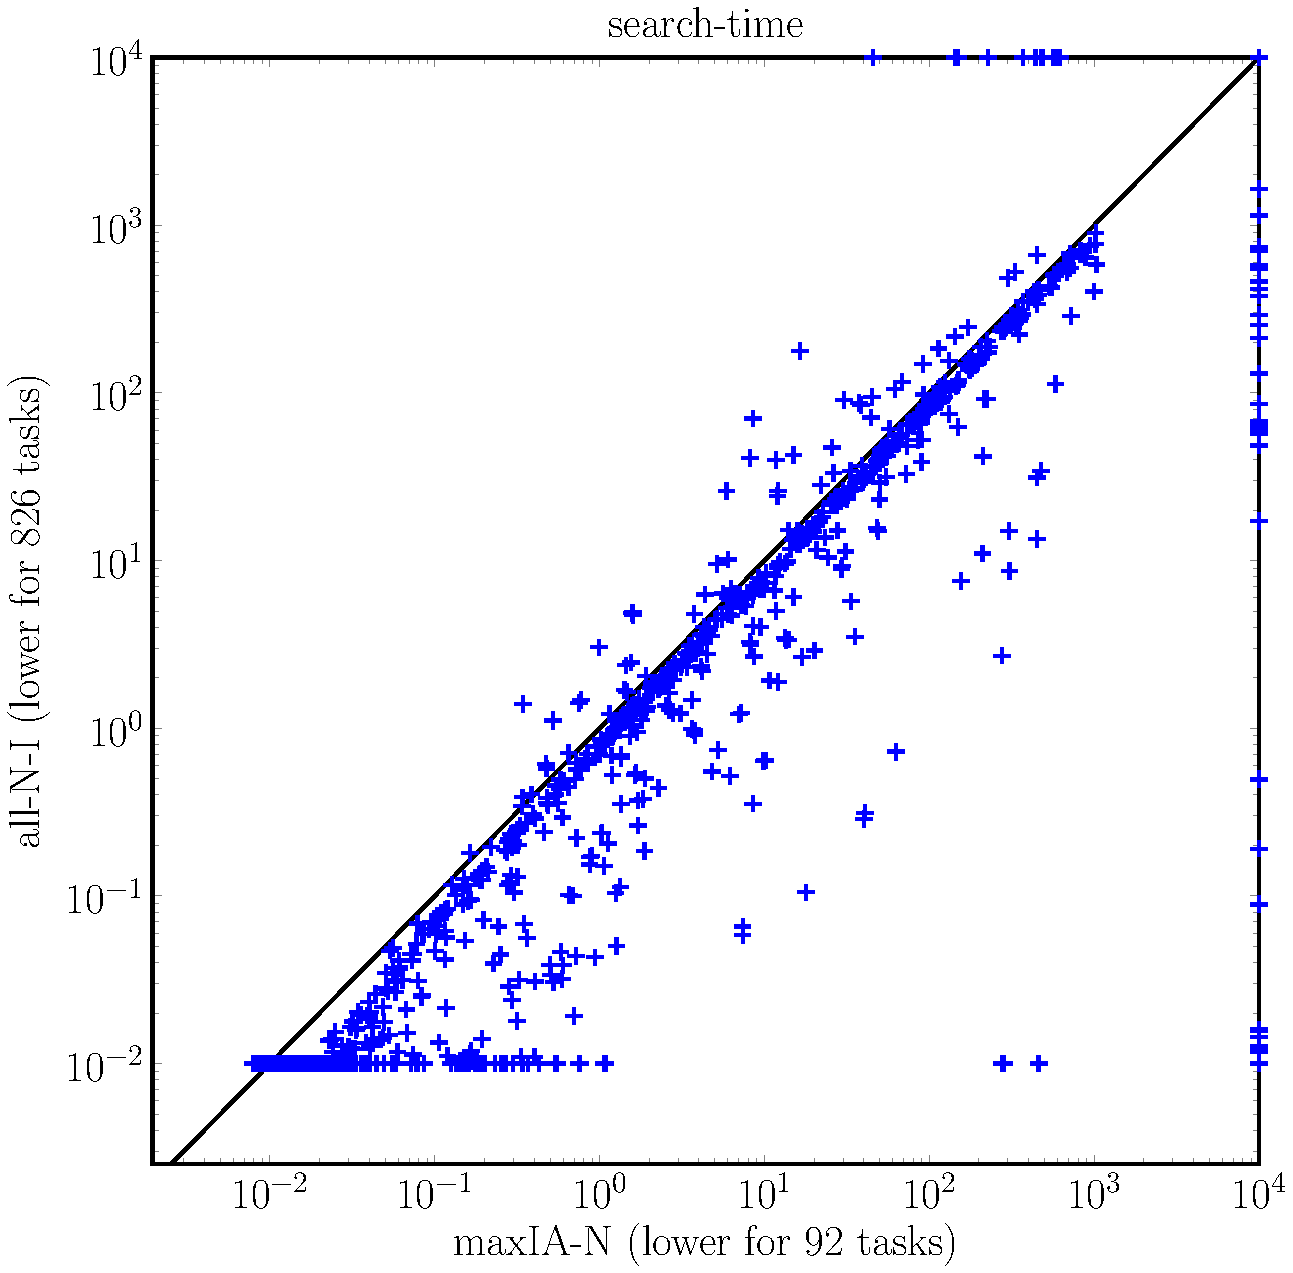
\includegraphics[width=0.5\textwidth]{all_max_search}
    \caption{Search Time  for \texttt{all} for both LPs per problem}
    \label{fig:search_max_all}
\end{figure}

\subsection{Additional Constraints on Random States}\label{subsec:additional-constraint-on-random-states}
In order to test the additional constraints on random states, we first tested different amounts of samples.
The pretests showed that 5 samples are best, which is why all following results are for $n=5$.

\begin{table}[h!]
    \begin{center}
        \begin{tabular}{|r|c|c|c|c|}
            \hline
            & \textbf{\texttt{all-N-R}} & \textbf{\texttt{init-N-R}} &\textbf{\texttt{div-N-R}} & \textbf{$\texttt{M}_\texttt{2}$\texttt{-D-R}} \\
            \hline \hline
            \textbf{Coverage}       & \textbf{930}  & 898           & 905   & 863 \\ \hline
            \textbf{Expansions}     & 11672         & 16182         & 11306 & \textbf{9190} \\ \hline
            \textbf{Total Time}     & \textbf{0.35} & 0.44          & 0.76  & 1.51 \\ \hline
            \textbf{Search Time}    & \textbf{0.34} & 0.44          & 0.76  & 1.37 \\ \hline
            \textbf{Out of Memory}  & 858           & 899           & 798   & \textbf{728} \\ \hline
            \textbf{Out of Time}    & 16            & \textbf{11}   & 105   & 205 \\ \hline
        \end{tabular}
        \caption{Test results for the additional constraints on random states.}
        \label{table:random-samples-constraint}
    \end{center}
\end{table}

In comparison to~\autoref{table:standard_heuristics}, the coverage is higher with the additional constraints, as can be seen in Table~\ref{table:random-samples-constraint}.
For \texttt{init-N-R} the number of expansions, search time and total time are better as well.
For all other listed configurations, these attributes are better without the additional constraints on random states.

As we only used 5 samples, this could be a coincidence.
A higher amount of samples would be better, since an outlier in the samples could then be compensated with the other sample states.
As is, with only 5 samples, if the random walk occurs in the wrong direction, the resulting potentials are distorted.
However, for more samples, building the LP is not feasible inside our time limit.
This is, because we implemented the additional constraint such that the Linear Program is optimized for one state after the other and the new constraint is added to the LP before optimizing for the next state.
Another solution, which could take more samples into account, would be to optimize the LP for multiple samples at a time, and then add their respective heuristic values to the solver as a constraint.

Taking mutexes and disambiguations into account when generating the samples could possibly enhance the result as well.

In Table~\ref{table:initial-random-samples-constraint}, the results for the combined additional constraints on the initial and on random states are listed.
The results are better compared to only using the constraints on random states, but still not as good as with the sole use of the constraint on the initial state.
In fact, all attributes lie between the configurations with only one type of additional constraints.

\begin{table}[h!]
    \begin{center}
        \begin{tabular}{|r|c|c|c|c|}
            \hline
            & \textbf{\texttt{all-N-I-R}} & \textbf{\texttt{div-N-I-R}} & \textbf{$\texttt{M}_\texttt{2}$\texttt{-D-I-R}} \\
            \hline \hline
            \textbf{Coverage}       & \textbf{963}  & 954  & 895   \\ \hline
            \textbf{Expansions}     & 8671          & 8897 & \textbf{6245}   \\ \hline
            \textbf{Total Time}     & \textbf{0.29} & 0.74 & 1.36  \\ \hline
            \textbf{Search Time}    & \textbf{0.29} & 0.74 & 1.24  \\ \hline
            \textbf{Out of Memory}  & 827           & 798  & \textbf{694}   \\ \hline
            \textbf{Out of Time}    & \textbf{26}   & 58   & 206   \\ \hline
        \end{tabular}
        \caption{ Test results for the combination of the additional constraints on the initial state and on random states.}
        \label{table:initial-random-samples-constraint}
    \end{center}
\end{table}

We also tested different variants of \texttt{max}.
Using \texttt{max} of \texttt{init} and \texttt{all} with the additional constraint on the initial state (\texttt{max(init-N, all-N-I)}), the coverage was 957 and therefore better than without the constraint.
It was a little lower with the additional constraints on random states for both \texttt{init} and \texttt{all} (\texttt{max(init-N-R, all-N-R)}, 927).
However, it was the only configuration, where the combined additional constraints yielded a better coverage, as the single use of the additional constraint of the initial state.
For \texttt{max(init-N-R, all-N-I-R)}, the coverage was 960.

\section{Comparison to Fi{\v{s}}er et al.}\label{sec:comparison-to-fiser}
In comparison to our results,~\cite{fivser2020strengthening} obtained a higher coverage using mutexes and disambiguations.
In order to find out why, we used their code (\texttt{cpddl}\footnote{https://gitlab.com/danfis/cpddl/}) for translating and pre processing the planning tasks and generating the potentials.
The potentials where then used in the Fast Downward $\textup{A}^\star$ search.
The results can be seen in Table~\ref{table:fiser}.

\begin{table}[h!]
    \begin{center}
        \begin{tabular}{|r|c|c|c|c|c|c|c|}
            \hline
            & \textbf{\texttt{all-N}} & \textbf{\texttt{all-D}} & \textbf{\texttt{max-D}} & \textbf{\texttt{div-D}} & \textbf{$\texttt{S}_\texttt{1000}^\texttt{1}$\texttt{-D}} & \textbf{$\texttt{M}_\texttt{1}$\texttt{-D}} & \textbf{$\texttt{K}_\texttt{1}^\texttt{50}$\texttt{-D}} \\
            \hline \hline
            \textbf{Coverage}       & 926       & 952       & 961   & 946           & 985   & \textbf{962}  & 923   \\ \hline
            \textbf{Expansions}     & 37795     & 29386     & 47314 & \textbf{24544}& 26908 & 31841         & 49766 \\ \hline
            \textbf{Total Time}     & 0.61      & 0.52      & 0.80  & \textbf{0.45} & 0.48  & 0.56          & 0.71  \\ \hline
            \textbf{Search Time}    & 0.54      & 0.46      & 0.71  & \textbf{0.40} & 0.42  & 0.49          & 0.63  \\ \hline
            \textbf{Out of Memory}  & 833       & 807       & 792   & \textbf{643}  & 770   & 791           & 812   \\ \hline
            \textbf{Out of Time}    & \textbf{2}& \textbf{2}& 5     & 92            & 3     & 5             & 5     \\ \hline
        \end{tabular}
        \caption{Test results obtained with \texttt{cpddl}}
        \label{table:fiser}
    \end{center}
\end{table}

For \texttt{all-N}, the coverage is worse than in our implementation.
All other configurations yield a higher coverage with \texttt{cpddl}.

Since \texttt{cpddl} uses a different preprocessor, we should not compare the relative attributes expansion, total time and search time with our former results.

What we can compare though are the out of time and out of memory errors.
That they are significantly lower than before, especially the out of time errors, indicates that \texttt{cpddl} is faster than our implementation.
As this holds for \texttt{all-N} as well, we can assume this is not only due to our implementation of the mutex calculation and the mutex based LP, but also due to the fact that \texttt{cpddl} uses a different preprocessor as Fast Downward.
